\documentclass[12pt]{article}
\usepackage{titlesec}
\usepackage{setspace}
\usepackage{graphicx}    % needed for including graphics e.g. EPS, PS
\usepackage[left=1.5in,top=1in,right=1in,bottom=1in]{geometry}
\textwidth 6in
\textheight 9in
%\pagestyle{empty}       % Uncomment if don't want page numbers
\parskip 7.2pt           % sets spacing between paragraphs
%\renewcommand{\baselinestretch}{1.5} % Uncomment for 1.5 spacing between lines
\parindent 0pt		 % sets leading space for paragraphs
\titleformat{\section}{\bfseries}{\thesection}{12pt}{}
\newcommand{\sectionbreak}{\clearpage}
\begin{document}         
% Start your text

\section{Abstract}
\label{Abstract}
\doublespacing

One of the most impressive qualities of the brain is it's plasticity. The neocortex has roughly the same structure throughout it's whole surface, yet it performs a variety of different tasks from vision to motor control, and regions which once performed one task, can learn to perform another. Any machine learning algorithm which claims to be a plausible model of the neocortex should also display this plasticity. One such candidate is the stacked de-noising autoencoder (SdA) It has shown promising results in the field of machine perception where it has been used to learn abstract features from unlabeled data. In this thesis, I use one possible unification of the process of perception and control to apply SdAs to a planning task in the game of Go. Planning is interpreted as the prediction of one's own actions with a bias towards desirable situations at all levels of abstraction.

\section{Motivation and outline of methods.}
\label{Motivation and outline of methods.}

It has been observed in psychology that eyewitness testimony is unreliable. People remember events with a self-serving and confirmation biases. They recall the world being closer to their own model than it really is, and their model is biased towards scenarios that would benefit them. I claim that this is an artifact of a beneficial adaptation: the brain's unification of perception and control in the neocortex. Under this hypothesis, we do not have a model of the world, and a set of goals from which we derive plans. We have a single biased model which simultaneously represents both imperfectly. This model is hierarchically organized into levels of abstraction. It is possible that the most abstract levels are more representative of goals than of the world, but each level is still permeated with bias to some extent.

Many unsupervised machine learning algorithms have been recently explored in the field of Deep Networks, which have been shown to be capable of learning hierarchies of abstraction to encode data. In this sense, the algorithms generalize. It remains to be seen whether these deep learning algorithms can be applied successfully to motor control, high-level planning, and the many other functions we know the neocortex is involved in. Moving forward in the search for artificial general intelligence it is important that we test new algorithms on the same variety of tasks as we know the brain to be capable of solving, and that we test them at the same scale in realistic environments, to the extent that sufficient computer power is affordable. A scalable algorithm which has mediocre performance on a variety of tasks with today's computing power is more promising as a model of the brain than an algorithm that excels at only one task.

In this thesis, I describe my experiments with with one deep learning algorithm, stacked de-noising auto-encoders, and my attempts to apply it to planning. I use one possible unification of the processes of perception and control in which a self-serving biased model of the world is trained on unlabeled data, and optimistic expectations of one's own future behavior are taken and directly acted out. For example, if such a model were being used to direct the motion of your arm, it might predict based on the inertia of your limbs and past associations between that inertia and self-observation of signals sent to the arm, that you were and will continue to be sending a pattern of muscle activation to the arm that would keep it moving in the same direction. But that prediction would be also biased towards patterns which move your arm towards the place you want it to be. At some level in your mental hierarchy, you believe your arm to be closer to it's goal than it actually is. This expectation gets propagated to other regions which take it for granted as ground truth, simply spitting out biased predictions of whatever they are sensitive to. Any region which observes and models the muscle activation signals sent out of the brain can double as a final decoder for turning expectations of arm positions into realistic goal-directed muscle stimulations.

I approximate this type of planning by training the highest layer of the SdA with a higher learning rate for games which resulted in a win for the player whose perspective the game is being observed from. I use a lower learning rate for moves in games which resulted in a loss. Lower layers are trained with a learning rate dependent on how close their activation was to the "goals" of the layer above, and the "observations" of the layer below, with the exception of the lowest layer, where it's activations do not vary from ground truth. Since, traditionally SdA's are trained by building up one level at a time, and my method requires information from higher levels to be present at the beginning, I use a hybrid approach where I build up a standard SdA one level at a time first, using constant learning rates from the level above, and then fine tune the entire network with the bias towards winning games, allowing progressively less abstract goals to propagate down the network as modified learning rates.

\section{Background on Auto-encoders}
\label{Background on Auto-encoders}

Autoencoders, or autoassociators as they are sometimes called, are a variant of the simple three-layer artificial neural network where the output is expected to equal the input and the hidden layer is smaller or sparser than than the input layer. An autoencoder takes an input $\mathbf x\in[0,1]^d$ and first maps it (with an encoder) to a hidden representation $\mathbf y\in[0,1]^{d'}$ through a deterministic mapping, e.g.:

\[
\mathbf y = s(\mathbf W\mathbf x + \mathbf b)
\]
Where $s$ is a non-linearity such as the sigmoid. The latent representation $\mathbf y$, or code is then mapped back (with a decoder) into a reconstruction $\mathbf z$ of same shape as $\mathbf x$  through a similar transformation, e.g.:
\[
\mathbf z = s(\mathbf W'\mathbf y + \mathbf b')
\]
$\mathbf z$ should be seen as a prediction, or {\it reconstruction}, of  $\mathbf x$ given the code  $\mathbf y$. The parameters of this model ($\mathbf W$, $\mathbf W'$, $\mathbf b$, and $\mathbf b'$) are optimized such that the average reconstruction error is minimized\cite{Bengio09}.

The aim of the autoencoder to learn the code $\mathbf y$ a distributed representation that captures the coordinates along the main factors of variation in the data (similarly to how principal component analysis (PCA) captures the main factors of variation in the data). Because $\mathbf y$ is viewed as a lossy compression of $\mathbf x$, it cannot be a good compression (with small loss) for all $\mathbf x$, so learning drives it to be one that is a good compression in particular for training examples, and hopefully for others as well, but not for arbitrary inputs. That is the sense in which an auto-encoder generalizes: it gives low reconstruction error to test examples from the same distribution as the training examples, but generally high reconstruction error to uniformly chosen configurations of the input vector.

If there is one linear hidden layer (the code) and the mean squared error criterion is used to train the network, then the  hidden units learn to project the input in the span of the first  principal components of the data. If the hidden layer is non-linear, the auto-encoder behaves differently from PCA, with the ability to capture multi-modal aspects of the input distribution. The departure from PCA becomes even more important when we consider stacking multiple encoders (and their corresponding decoders) when building a deep auto-encoder [Hinton06].

The auto-encoder alone is not sufficient to be the basis of a deep architecture because it has a tendency towards over-fitting. The denoising autoencoder (dA) is an extension of a classical autoencoder introduced specifically as a building block for deep networks\cite{Vincint08}.  It attempts to re-construct a corrupted version of the input, but the error in $\mathbf z$ is still compared against the un-corrupted input. The stochastic corruption process consists in randomly setting some of the inputs (as many as half of them) to zero. Hence the denoising auto-encoder is trying to predict the corrupted (i.e. missing) values from the uncorrupted (i.e., non-missing) values, for randomly selected subsets of missing patterns. This modification allows the dA to generalize well and produces compounding benefits when the dA's are stacked into a deep network\cite{Hinton06}. Hinton (google tech talk 3) suggests that the stochastic timing of the action potentials observed in biological neurons is a similar feature evolved to moderate the potential for over-fitting, and allow neurons or neuron groups to generalize well over the range of activation patterns of their receptive fields.

\section{0.1 Stacked de-noising autoencoders}
\label{Stacked de-noising autoencoders}

Stacked denoising autoencoders, canonically abbreviated SdA, are not just neural networks with additional hidden layers, but a structure with individual levels of simple three-layer denoising autoencoders. First, a single denoising autoencoder is trained on the data. It's hidden layer converges on a sparse distributed representation of the training set. This essentially replaces the step where a researcher would have to design a collection of good features. Then, a second denoising autoencoder is trained to reconstruct corrupted versions of the activation of the hidden layer of the first dA for the collection of training examples. (the first level does not learn during this time). After a sufficient number of levels have been added, if the network is to be used for classification, the encoders and decoders from each level are assembled into one long network and fine-tuned using back-propagation.

Jeff Hawkins said in 2004, "Neural networks were a genuine improvement of the AI approach because their architecture is based, though very loosely, on real nervous systems...But as the neural network phenomenon exploded on the scene, it mostly settled on the class of ultra-simple models that didn't meet any of [his criteria for biological plausibility]. Most neural networks consisted of a small number of neurons connected in three rows...I thought the field would quickly move on to more realistic networks, but it didn't. Because these simple neural networks were able to do interesting things, research seemed to stop there for years." \cite{Hawkins04} I agree with this sentiment, but at this point we are finally moving past simple networks and building large systems out of several smaller neural networks. One day, computer power permitting, collections of SdAs and other types of deep networks will be used together in even larger systems to accomplish more impressive feats of AI.

\begin{figure}[htb]
\begin{center}
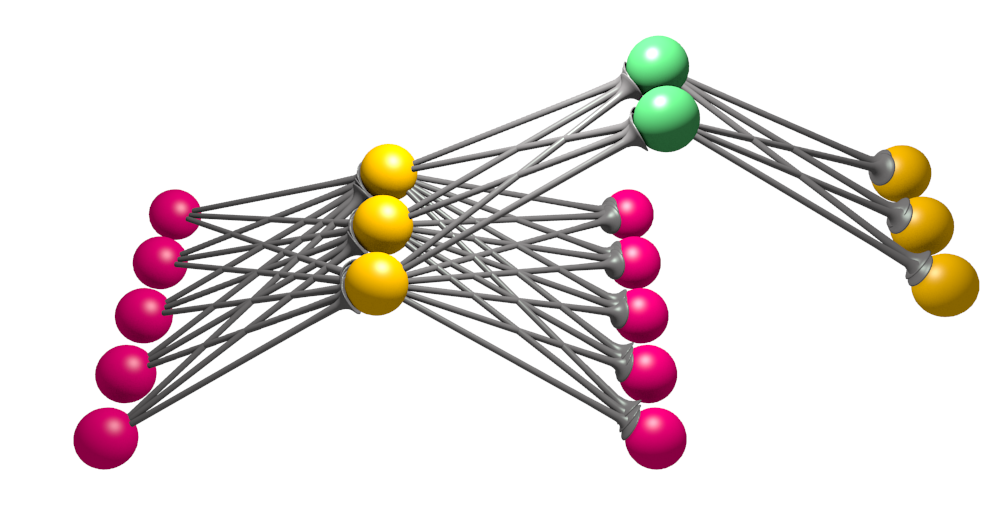
\includegraphics[height=2.585in,width=5in]{sda_fig}
\caption{An SdA with two autoencoders. Each autoencoder is a a simple three layer network. The input/output to the first layer is the pink level, and the yellow level is it's distributed code, or hidden layer. The yellow hidden layer is then used as input/output to another autoencoder, it's hidden layer is shown in green.}
\end{center}
\end{figure}

The reason deep belief networks offer some benefit over a completely flat network with the same number of trainable parameters is that they can generalize at different levels and thus share more information. For example, a flat network which has learned a mapping between pictures of cars and labels cannot re-use any of those weights to learn a mapping between pictures of animals and labels. However, a deep network with an intermediate layer sensitive to edges could be shared between them and both classifiers could then be expressed with a far smaller number of weights, as all natural images can be more compactly represented as collections of edges. 

\section{1.0 Successes of SdAs on machine perception tasks}
\label{Successes of SdAs on machine perception tasks}

Deep belief nets (including SdAs and Stacked Restricted Boltzmann Machines) have been used for generating and recognizing images (Hinton, Osindero \& Teh 2006, Ranzato et. al. 2007, Bengio et.al., 2007), video sequences (Sutskever and Hinton, 2007), and motion-capture data (Taylor et. al. 2007)

The largest experiment so far with an SdA, by Google, was able to learn feature detectors for the human face, and a cat by training on 10 million images taken from youtube videos\cite{Le12}. They used 4 levels of autoencoders. Some other steps were used as well, such as local contrast normalization and local max pooling, a standard procedure in machine vision. They trained the network for three days on a cluster with computing power in the neighborhood of 1 PFLOP.

Training neural networks is an easy process to parallelize and distribute across many computers. However, all the extra training that occurs in an SdA requires even more computer power than usual. The de-noising step slows down convergence, and in order to converge to the same level as without it, the number of training cycles must be increased by roughly an order of magnitude. For this reason, and because of falling costs, the latest developments in SdAs have been run on GPUs. Nvidia's CUDA shader language combined with a top of the line GPU (or several) affords 10 to 1000 fold increases in speed for applications which can fit in GPU memory. Using Python and Theano\cite{Bergstra10}, a binding to the GPU accelerated linear algebra library LAPACK on Ubuntu, and a single Nvidia GTX 570 capable of 1405 GFLOPS, I was able to achieve about 20x increase in speed on a simple SdA pre-training operation on the MINST dataset, over a quad-core Intel i5-2500k CPU at 4.5 Ghz, measured to be capable of only 59 GFLOPS.

\section{1.1 Applications of SdAs to planning tasks}
\label{Applications of SdAs to planning tasks}

The essence of planning is the attainment of a goal through a series of intermediate steps which do not necessarily lead directly toward that goal\cite{Baker95}. Various kinds of neural network based models have been applied to planning tasks, but SdA's are not among them. 

Self-Organizing Maps (SOM) were used by Anmin Zhu to control robot swarms. 

Classic explicit planning systems which represent actions as symbols selected from a finite list, have been modified to have hierarchies of abstraction by (Knoblock 1991) and later by (Boutilier \& Dearden 1994). This saves on search time by reducing the size of the search space, as some actions have similar outcomes, and can be effectively reasoned about by grouping them into an abstract class.



\section{2.0 Plausibility of SdA's as a model of the mammalian neocortex}
\label{Plausibility of SdA's as a model of the mammalian neocortex}

The primate visual cortex is one of the most studied brain regions in the animal kingdom. We know that it is composed of several levels, each more abstract than the one before it. The cortical columns in V1 are sensitive to a small receptive field of light coming in from the lateral genticulate cortex, which in turn receives information from the optic nerve. They are each slightly sensitive to certain angles and colors more than others. V2, which has connections drawing from V1 and other areas, has cells that are sensitive to mildly complex shapes somewhat invariant to translation, rotation, and scale, and will detect these shapes within a slightly larger receptive field. This gradual increase in abstraction continues as you move up the chain of levels, until you have neurons that are sensitive to something invariant like "person" or "thing moving towards me at an alarming speed"

The SdA method is evolving with functionality and performance in mind, and not explicitly to mimic the cortex, but we find that it has many of the same strengths and weaknesses. One such strength is it's plasticity. An SdA pre-trained to see video, performed better at a hearing task after fine-tuning, than a randomly initialized network fine-tuned in the same way. This is presumably because sound and video share some macro-statistical properties, such as having a high kurtosis.

An SdA also goes through different phases of learning that resemble the phases in a person's maturation. We know that plasticity in the brain decreases over time, and at about 30, the brain changes over to a new mode where it begins to fine tune existing connections and grows almost no new connections in the cortex.

\section{2.1 Philosophical points}
\label{Philosophical points}

The levels in the SdA are levels of abstraction. What are the implications of a possible root at the top of this tree?

Perception is like nested stack of expectations, specific expectations of the near future based on a deluge of sensory data, and a smaller collection of abstract expectations of the medium range future based on a shower of specific, short-range expectations and some more sensory data. Recurse until lost.

Does this tree have a root? is there some "most abstract representation" of our sensory experience that we can expect in the indefinitely long run, that decodes to the specifics that we will in fact observe from this point on? I think that this very theory is a candidate. But that's not as important as it sounds. What any abstract expectation actually predicts depends on the more specific models below it, and the sensory data yet to be observed.  "This too shall pass" would make a perfectly good root for our tree, if giving it that role didn't actually turn it into a paradox. A root here is really not more important than a leaf.

Let me re-iterate. I am operating on the assumption for this project, that perception and planning are both part of the same process, so the most abstract representations are joint models of sensory experience and action. The model of sensory data is influenced by three main factors. The accuracy, the sparsity, and the desirability, or pleasurableness to the creature. At all levels, the representations which jointly satisfy these three metrics come to dominate. In the case of a game this last factor would be the points or wins/losses experienced by the player. The player perceives the state of the game and the state of it's own recent actions, and expects a likely, sparse, and desirable scenario next, and then is made to take any actions it expected of itself which are legal in the rules of the game. It may not be the most brilliant way to play a game, but I think It would at least perform OK at Puerto Rico, a game about economic growth.



\section{3.0 Expected performance of SdA vs greedy approach}
\label{Expected performance of SdA vs. dA}

The SdA's layered hierarchy of abstraction could theoretically allow it to outperform the greedy approach, if the problem space is decomposable into abstract levels, which from play experience, I believe it is. The situations in which a greedy approach would fail to an algorithm that has more high-level concerns besides points gained on the next turn are ones in which sacrifice is useful or more commonly, ones in which delayed capture of a group would leave open the opportunity for additional enemy mistakes, and therefore, more captures.

A simple greedy hill climbing go engine was used as a control opponent (SimpleGo 0.1.X). It always makes the move which would maximize it's relative capture point gain on the next turn, and if that cannot be improved, maximizes it's relative advantage in total liberties.

\section{3.2 Training the SdA}
\label{Training the SdA}

To construct the dataset, I first collected tens of thousands of recorded go games as SGF files from the IGS server and other sources such as professional tournaments. I then filtered out about 20 percent of those games because they were in incomplete or were played by nonstandard rules. Then each move in each games was recorded as a training example. Training examples were vectors of 363 numbers between 0 and 1. The first 361 numbers were the board positions of the 19x19 board. an empty position was represented with 0.5, while a white or black stone was represented with 0.75 or 0.25 respectively. The last moves of white and black were represented with 0 and 1 respectively. I chose not to represent the last moves as normalized coordinates because that would make them sensitive and would create a very non-smooth space for the most important parameters in the model. Finally, the last two numbers are the normalized clamped game move number and the final score for black. In each game, the moves of both players are used to create training examples but white's moves are inverted because all moves are stored from black's perspective and when the engine plays go, if it plays as white, it inverts the state to present it to the SdA.

Overall, 1.9 million training examples were created. This dataset was then divided randomly into training, test, and validation sets. 4/5ths of the initial set was used as training data, 4/5ths of what remained was test data, and the remaining part was the validation set. The dataset could not fit in main memory so it was randomized using parallel external merge sort of murmur3 hashes of the training example indices plus a constant seed offset. The randomized data were divided into 1 Gb chunks and stored on an SSD for fast loading into the GPU.

The SdA was pre-trained on a dataset of 1,922,933 go positions from the color perspective of the winner. Only the moves in which the winner just places a stone were used. This is the sense in which the SdA preferentially remembers desirable situations, as opposed to remembering all situations in an unbiased model of reality and then deriving actions from the model and a goal. One attempt was made to modify the learning rate with respect to the game's final score on a point by point basis, but it was core-limited as it required communication between the CPU and GPU on every data point, and at the speed of one core, the training process would not have finished for several months. In order to fully take advantage of the GPU and finish in a reasonable amount of time, additional optimizations would have to be designed specifically for this application.

The network topology used was [363, 250, 150, 50, 10]. Each denoising autoencoder in the SdA was trained for 100 iterations of the entire dataset. The entire SdA has about $\mathbf 2^{18}$ trainable parameters. One interesting thing we can do with the fully trained encoder is to look at each of the 10 highest level hidden units, and look at what kind of Go board it is maximally activated by. To do this, we set it's activation to 1, and set the activation of the other high-level hidden units to 0, then use the series of decoders on the lower levels to construct a low-level training example. this example can be then passed into a drawing program to represent it's weights on a go board.

\begin{figure}[htb]
\begin{center}
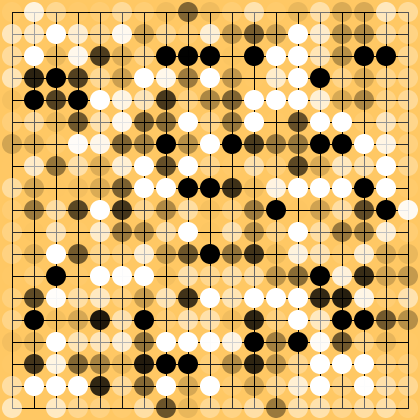
\includegraphics[height=3.0in,width=3.0in]{screen-0204}
\caption{A representation of the go position that would maximally activate one of the hidden units from the highest level in the SdA. Stones are either colored white or black based on the direction of the prediction, and the opacity is the confidence that a stone would be in that position rather than being empty.}
\end{center}
\end{figure}

\section{3.1 Implementation of Go Engine}
\label{Implementation of Go Engine}

A standard go engine is a computer program which can speak GTP (Go Text Protocol) and decide on moves from game states. Through a bit of wrapper code, it connects to a go server like KGS or a local game arbitration software where it plays games against humans or other go engines. I used an excellent local go engine manager and go library called Gomill by Matthew Woodcraft.

The go engines takes a game state from the current game, and creates a vector of floats from it in the same way that the dataset training examples were created. An empty space is represented as a 0.5, a stone of one's own color represented with a 0.25, a stone of the other player represented with a 0.75. Ones own last move (in the training examples) is represented with 0.0 and the opponents last move with a 1.0. There are two other numbers added. the move number / 200 and the final score from one's own color's perspective. The SdA's encoder weights are used to propagate the activations up to the highest hidden layer, and then the decoder weights are used to propagate those activations back down to the board's state. It is hoped that the resulting prediction will resemble the board state the network was primed with, plus the information about the "last move" made by the current player, which was always present in the training data. At this point, the legal board position with the minimum predicted value is taken to be the choice move and the play is made. The Gomill library handles the GTP protocol from there on.

Why was Go chosen? it is a difficult game for computers, with a huge branching factor. This ensures that brute force is infeasible and rules out the possibility of it being used in-whole or in-part. Go requires planning at different scales of time and space. Sometimes sacrifice is strategic. Neither a purely greedy or purely sustainable outlook is as good as a balance between the two.

\section{4.0 Performance of SdA-based player against dA player and various other opponents}
\label{Performance of SdA-based player against dA player and various other opponents}

performance matrix?
SdA vs. single layer dA
SdA vs. Greedy Approach
SdA vs. GNU Go level 1

\section{Analysis of the behavior of trained SdA}
\label{Analysis of the behavior of trained SdA}

By observing played games, creating visualizations of the hidden nodes in the network, we can try to get an idea of how the SdA is encoding the data, and whether it has converged on abstract representations of typical Go patterns, and whether it can be said to have "plans".

\section{4.1 Conclusion and lessons learned}
\label{Conclusion and lessons learned}




\begin{thebibliography}{99}
\singlespacing

\bibitem{Baker95} S. C. Baker, R. D. Rogers, A. M. Owen, C. D. Frith, R. J. Dolan, R. S. J. Frackowiak, T. W. Robbins. Neural systems engaged by planning: a PET study of the Tower of London task. Neuropsychologia,Vol. 34, No. 6, pp. 515-526, 1996
 
\bibitem{Bengio07} Bengio, P. Lamblin, D. Popovici and H. Larochelle, Greedy Layer-Wise Training of Deep Networks, in Advances in Neural Information Processing Systems 19 (NIPS�06), pages 153-160, MIT Press 2007.
 
\bibitem{Bengio09} Bengio, Learning deep architectures for AI, Foundations and Trends in Machine Learning 1(2) pages 1-127.

\bibitem{Hawkins04} Jeff Hawkins and Sandra Blakeslee. On Intelligence. Times Books, 2004.

\bibitem{Hinton06} G.E. Hinton and R.R. Salakhutdinov, Reducing the Dimensionality of Data with Neural Networks, Science, 28 July 2006, Vol. 313. no. 5786, pp. 504 - 507.

\bibitem{Hinton07} G.E. Hinton, S. Osindero, and Y. Teh, �A fast learning algorithm for deep belief nets�, Neural Computation, vol 18, 2006

\bibitem{Bergstra10} J. Bergstra, O. Breuleux, F. Bastien, P. Lamblin, R. Pascanu, G. Desjardins, J. Turian, D. Warde-Farley and Y. Bengio. �Theano: A CPU and GPU Math Expression Compiler�. Proceedings of the Python for Scientific Computing Conference (SciPy) 2010. June 30 - July 3, Austin, TX

\bibitem{Le12} Quoc Le, Marc'Aurelio Ranzato, Rajat Monga, Matthieu Devin, Kai Chen, Greg Corrado, Jeff Dean, Andrew Ng. Building high-level features using large scale unsupervised learning. International Conference in Machine Learning, 2012.

\bibitem{Ranzato06} Marc�Aurelio Ranzato, Christopher Poultney, Sumit Chopra, and Yann LeCun. Efficient Learning of Sparse Representations with an Energy-Based Model. Advances in Neural Information Processing Systems, 2006.

\bibitem{Vincint08} Vincent, H. Larochelle Y. Bengio and P.A. Manzagol, Extracting and Composing Robust Features with Denoising Autoencoders, Proceedings of the Twenty-fifth International Conference on Machine Learning (ICML�08), pages 1096 - 1103, ACM, 2008.
 
\end{thebibliography}
\end{document}








